\documentclass[11pt]{article}
\usepackage{amsmath,amsbsy,amssymb,verbatim,fullpage,ifthen,graphicx,bm,amsfonts,amsthm,url}
\usepackage{graphicx}
\usepackage{xcolor}
%\usepackage[dvipsnames]{xcolor}
\usepackage{algpseudocode}
% \usepackage{xcolor}
\usepackage{listings}

\definecolor{codegreen}{rgb}{0,0.6,0}
\definecolor{codegray}{rgb}{0.5,0.5,0.5}
\definecolor{codepurple}{rgb}{0.58,0,0.82}
\definecolor{backcolour}{rgb}{0.95,0.95,0.92}

\lstdefinestyle{mystyle}{
    backgroundcolor=\color{backcolour},   
    commentstyle=\color{codegreen},
    keywordstyle=\color{magenta},
    numberstyle=\tiny\color{codegray},
    stringstyle=\color{codepurple},
    basicstyle=\ttfamily\footnotesize,
    breakatwhitespace=false,         
    breaklines=true,                 
    captionpos=b,                    
    keepspaces=true,                 
    numbers=left,                    
    numbersep=5pt,                  
    showspaces=false,                
    showstringspaces=false,
    showtabs=false,                  
    tabsize=2
}
\lstset{style=mystyle}

\usepackage{algpseudocode}
\newcommand{\mfile}[1]  {{\small \verbatiminput{./#1}}} % Jeff Fessler, input matlab file
\newcommand{\tmop}[1]{\ensuremath{\operatorname{#1}}}
\newcommand{\R}{\mathbb{R}}
\newcommand{\C}{\mathbb{C}}
\newcommand{\Z}{\mathbb{Z}}
\newcommand{\A}{\mathcal{A}}
\newcommand{\minimize}{\operatorname*{minimize\ }}
\newcommand{\maximize}{\operatorname*{maximize}}
\newcommand{\opdet}[1]{\operatorname{\textbf{det}}\left(#1\right)}
\newcommand{\optr}[1]{\operatorname{\textbf{tr}}\left(#1\right)}
\newcommand{\answer}[2][blue]{\ifdefined\AnswerDefine{\color{#1}\it#2}\fi}
\newcommand{\mtx}[1]{\mathbf{#1}}
\newcommand{\vct}[1]{\mathbf{#1}}
\def \lg       {\langle}
\def \rg       {\rangle}
\def \mA {\mtx{A}}
\def \mB {\mtx{B}}
\def \mI {\mtx{I}}
\def \mJ {\mtx{J}}
\def \mU {\mtx{U}}
\def \mS {\mtx{S}}
\def \mV {\mtx{V}}
\def \mW {\mtx{W}}
\def \mLambda {\mtx{\Lambda}}
\def \mSigma {\mtx{\Sigma}}
\def \mX {\mtx{X}}
\def \mY {\mtx{Y}}
\def \mZ {\mtx{Z}}
\def \zero     {\mathbf{0}}
\def \vzero    {\vct{0}}
\def \vone    {\vct{1}}
\def \vu {\vct{u}}
\def \vv {\vct{v}}
\def \vx {\vct{x}}
\def \vy {\vct{y}}
\def \vz {\vct{z}}
\def \vphi {\vct{\phi}}
\def \vmu {\vct{\mu}}
\def \R {\mathbb{R}}


\usepackage{xspace}
\makeatletter
\DeclareRobustCommand\onedot{\futurelet\@let@token\@onedot}
\def\@onedot{\ifx\@let@token.\else.\null\fi\xspace}

\def\eg{\emph{e.g}\onedot} \def\Eg{\emph{E.g}\onedot}
\def\ie{\emph{i.e}\onedot} \def\Ie{\emph{I.e}\onedot}
\def\cf{\emph{c.f}\onedot} \def\Cf{\emph{C.f}\onedot}
\def\etc{\emph{etc}\onedot} \def\vs{\emph{vs}\onedot}
\def\wrt{w.r.t\onedot} \def\dof{d.o.f\onedot}
\def\etal{\emph{et al}\onedot} \def\st{\emph{s.t}\onedot}
\pagestyle{plain}

\title{{\bf Homework Set 3, CPSC 8420, Fall 2024}} % Change to the appropriate homework number
\author{\Large\underline{Yarui Cao}}
\date{\textbf{\Large\textcolor{red}{Due 11/11/2024, 11:59PM EST}}} % put your name in the LastName, FirstName format
%\date{\today}

\begin{document}
	\maketitle
	

	%\section*{Problem 1}
\section*{Problem 1}
Please download the image from \url{https://en.wikipedia.org/wiki/Lenna#/media/File:Lenna_(test_image).png} with dimension $512\times512\times3$. Assume for each RGB channel data $X$, we have $[U,\Sigma,V]=svd(X)$. Please show each compression ratio and reconstruction image if we choose first $2, 5, 20, 50,80,100$ components respectively. Also please determine the best component number to obtain a good trade-off between data compression ratio and reconstruction image quality. (Open question, that is your solution will be accepted as long as it's reasonable.)

\textcolor{red}{Answer:}\\
The code for this problem is as follows:
\begin{lstlisting}[language = matlab]
	clear all; close all;

    ks = [2, 5, 20, 50, 80, 100];
    img = imread("Lenna.png");
    image = im2double(img);
    
    [m, n, channel] = size(img);
    
    for k = 1:length(ks)
        rec = reconstruction(image, channel, ks(k));
        rec = im2uint8(rec);
        compression_ratio = (m*k+k*k+k*n) / (m*n);
        % plot
        ax = subplot(2,3,k);
        imshow(rec, 'Parent', ax);
        title(ax, sprintf("first %d components,\n compression ratio=%.3f", ks(k), compression_ratio))
    end
    
    function image_rec = reconstruction(image, channel, k)
        image_rec = zeros(size(image));
        for ch = 1:channel
            X = image(:,:,ch);
            [U, S, V] = svd(X);
            X_rec = U(:, 1:k) * S(1:k, 1:k) * V(:, 1:k)';
            image_rec(:,:,ch) = X_rec;
        end
    end
    
\end{lstlisting}
The reconstruction images are shown in Fig.~\ref{fig:rec}. I'd select the first 50 components to reconstruct the image, as 50 is the smallest number among these six options that achieves good image quality.
\begin{figure}[h]
    \centering
    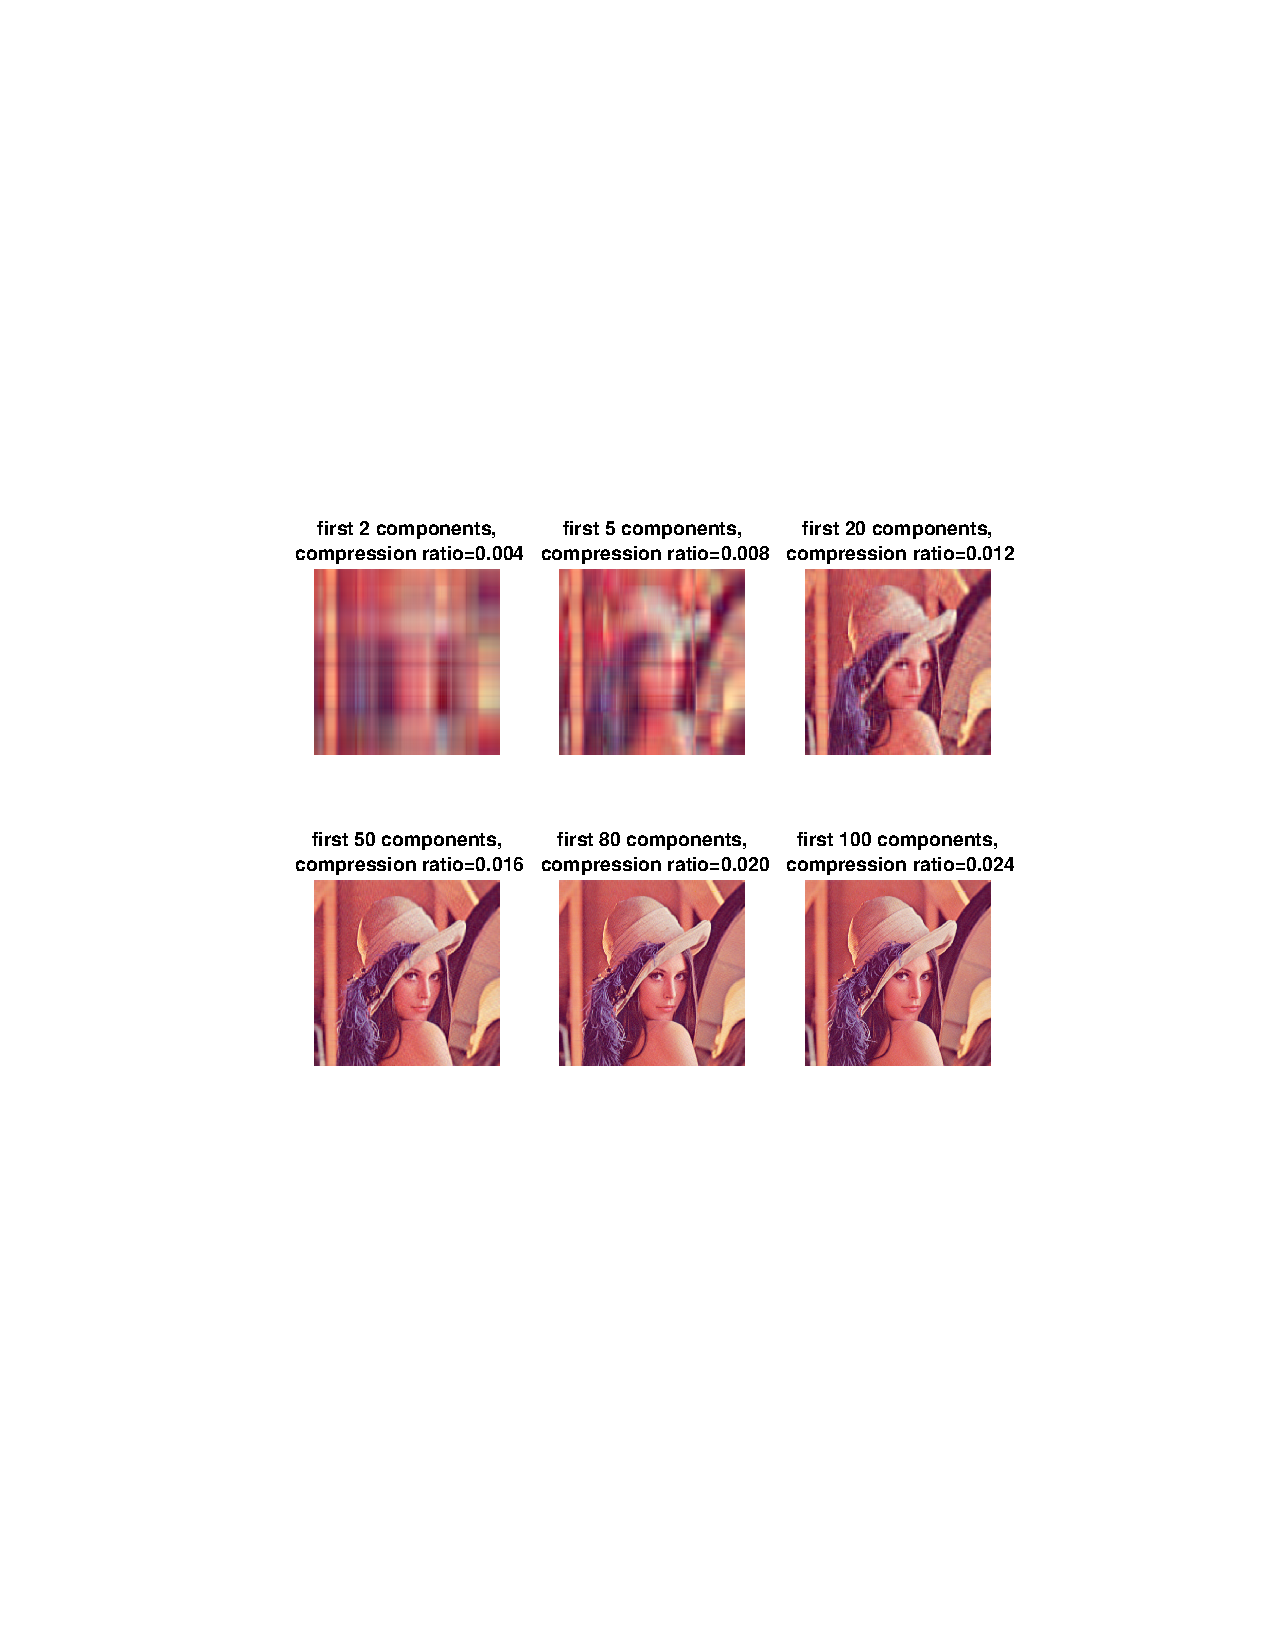
\includegraphics[width=0.95\linewidth]{Lena.pdf}
    \caption{Reconstruction images}
    \label{fig:rec}
\end{figure}





\end{document}
